\documentclass[12pt, a4paper]{article}
% Zobrazení frame - pro debug
%\usepackage{showframe}
\usepackage{lmodern}
\usepackage[czech]{babel}
\usepackage[T1]{fontenc}
\usepackage[utf8]{inputenc}
\usepackage{graphicx}
\usepackage{pdfpages}
\usepackage{amsmath}
\usepackage{xcolor}
\usepackage{listings}
\lstset{basicstyle=\ttfamily,
  showstringspaces=false,
  commentstyle=\color{red},
  keywordstyle=\color{blue},
  inputencoding=utf8,
  extendedchars=true,
  literate=%
    {á}{{\'a}}1
    {č}{{\v{c}}}1
    {ď}{{\v{d}}}1
    {é}{{\'e}}1
    {ě}{{\v{e}}}1
    {í}{{\'i}}1
    {ň}{{\v{n}}}1
    {ó}{{\'o}}1
    {ř}{{\v{r}}}1
    {š}{{\v{s}}}1
    {ť}{{\v{t}}}1
    {ú}{{\'u}}1
    {ů}{{\r{u}}}1
    {ý}{{\'y}}1
    {ž}{{\v{z}}}1
    {Á}{{\'A}}1
    {Č}{{\v{C}}}1
    {Ď}{{\v{D}}}1
    {É}{{\'E}}1
    {Ě}{{\v{E}}}1
    {Í}{{\'I}}1
    {Ň}{{\v{N}}}1
    {Ó}{{\'O}}1
    {Ř}{{\v{R}}}1
    {Š}{{\v{S}}}1
    {Ť}{{\v{T}}}1
    {Ú}{{\'U}}1
    {Ů}{{\r{U}}}1
    {Ý}{{\'Y}}1
    {Ž}{{\v{Z}}}1
}
\begin{document}

% Pouze informace
\graphicspath{ {img/} }

% Úvodní stránka
\thispagestyle{empty}
\begin{center}
\begin{minipage}{0.75\linewidth}
    \centering
%University logo
    \vspace{3cm}
    
\includegraphics[width=0.75\linewidth]{fav-logo.pdf}\\
    \vspace{0.5cm}
%Thesis title
    {\Large KIV/ZOS \\ \textbf{IMPLEMENTACE SYMETRICKÉ BLOKOVÉ ŠIFRY AES}\par}
    \vspace{4cm}
%Author's name
    {\Large Jakub Vítek (viteja) - A19B0222P\par}
    \vspace{2cm}
%Degree
    \vspace{2cm}
%Date
    {\Large Květen 2020}
\end{minipage}
\end{center}
\clearpage
\newpage

% Část obsahu dokumentu
\tableofcontents
\newpage

\addcontentsline{toc}{section}{Zadání}
\shorthandoff{-}
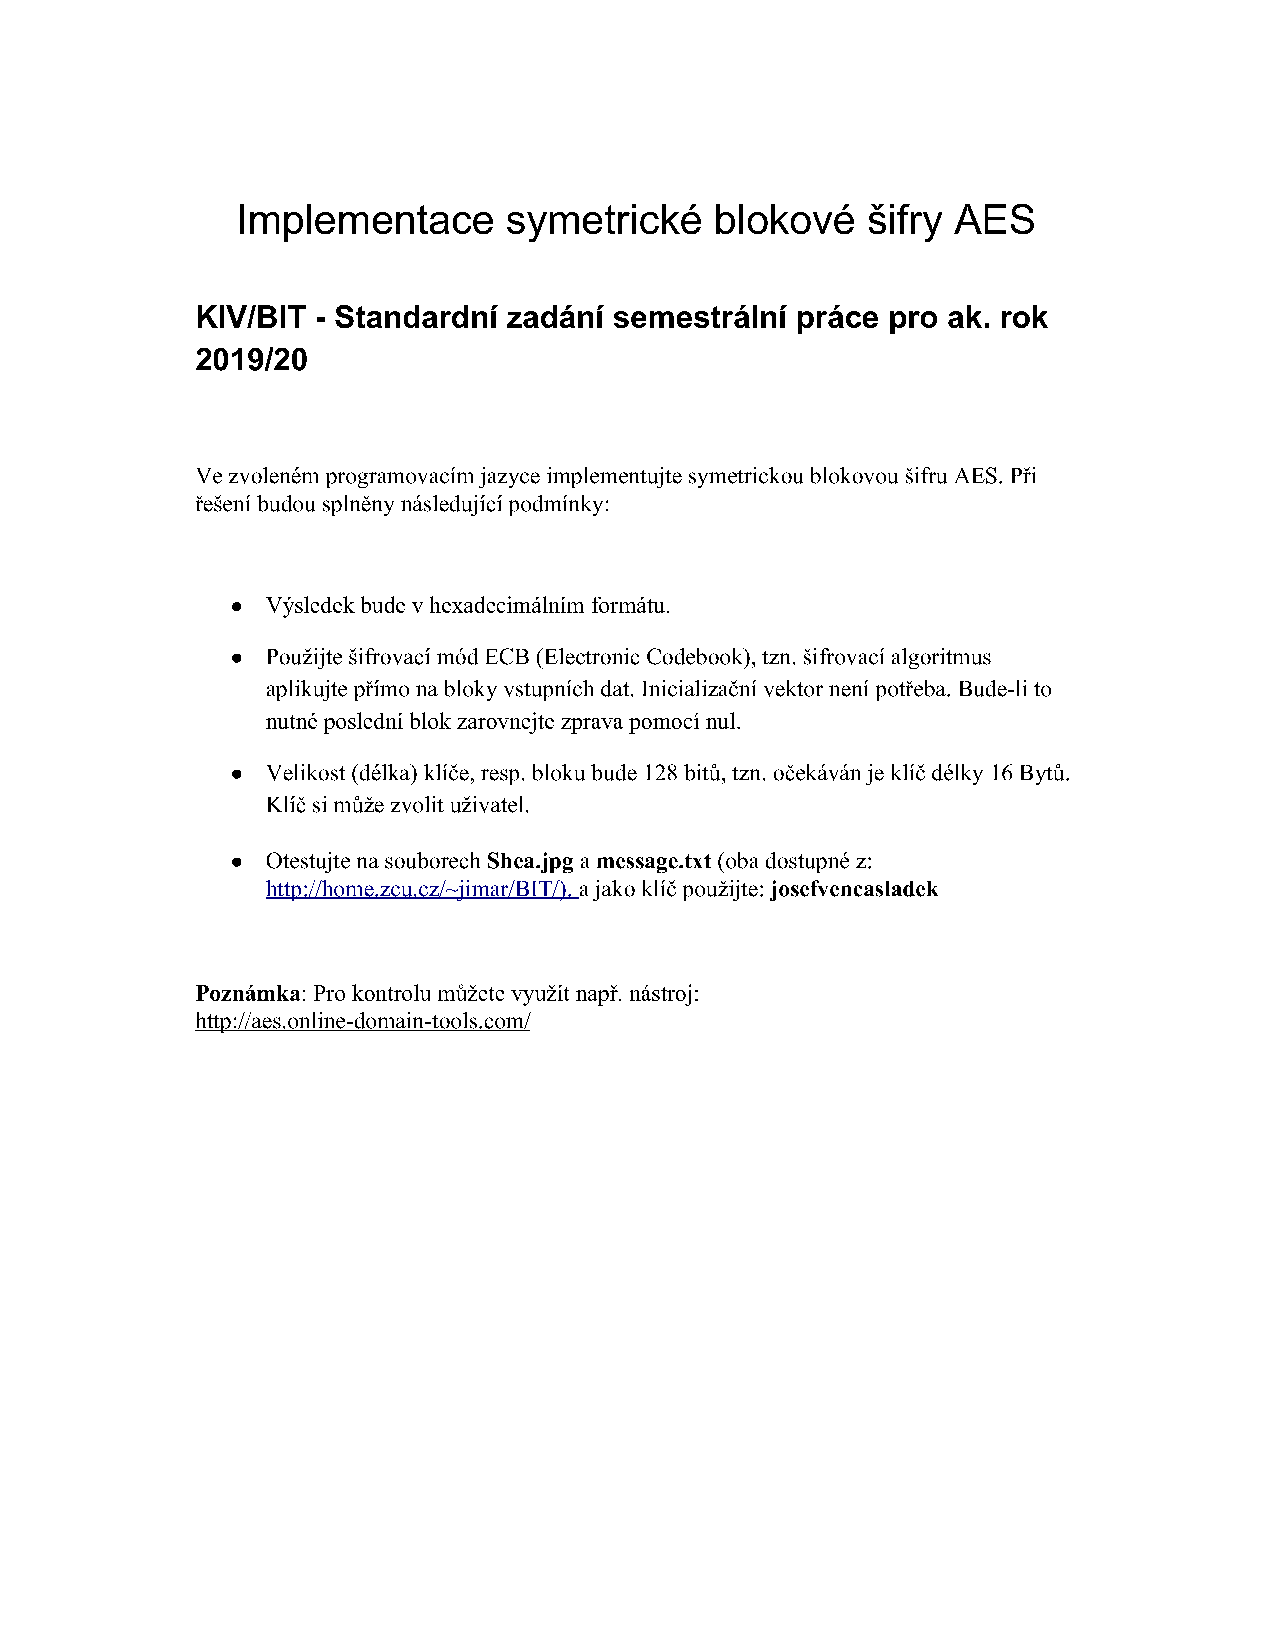
\includepdf[pages=-]{./include/zadani.pdf}
\shorthandon{-}


\section{Advanced Encryption Standard}
\paragraph{}
Advanced Encryption Standard je standardizovaným algoritmem pro šifrování dat informatice. Jedná se
se o symetrickou šifru, šifrování i dešifrování se provádí stejným klíčem.
\paragraph{}
Standardně, šifrování i dešifrování probíha nad bloky dat ve velikosti 128 bit (16 Byte). U klíče jsou pak vyžadovány
bloky velikostí 128 bit (16 Byte), 196 bit (24 Byte) či 256 bit (32 Byte). Algoritmus může pracovat ve dvou
základních režimech, kdy v režimu ECB (Electronic Codebook) jsou všechny bloky dat při šifrování na ostatních
blocích nezávislé a v režimu CBC (Cipher block chaining) je šifrování následujícího bloku parametrizováno výsledkem
šifrování bloku předchozího.
\paragraph{}
AES má relativně jednoduchý algebraický popis, z tohoto důvodu v minulosti proběhlo velké množství útoků na tuto šifru,
výsledkem těchto útoků bylo snížení složitosti při prolomení metodou brute force. I tak však algoritmus zůstává dostatečně
bezpečný a je v současné době používán pro zabepečení Wi-Fi sítě (WPA2). Výkon algoritmu je pak zajištěn podporou pro
jeho vnitřní operace v dnešním hardware.

\newpage
\section{Analýza}
\paragraph{}
Algoritmus AES pracuje s bloky dat ve velikosti 128 bit (16 Byte). Tyto bytes jsou uspořádány do matice o rozměrech
4x4 byte. Zadáním semestrální práce je dána nutnost použití klíče o velikosti 128 bit (16 byte). Standard algoritmu
pak říká, že pro klíč o velikosti 128 bit použijeme 10 iterací algoritmu. V rámci práce budeme používat šifrovací režim
ECB (Electronic Codebook), kdy budeme s každým blokem dat pracovat nezávisle na všech ostatních blocích dat.
\paragraph{}
V základu algoritmus pracuje na bázi substitucí, kdy nahrazujeme vstupní data výstupními a permutací, kdy měníme pozici
dat v logické struktuře (4x4 byte matice). V algoritmu jsou obsaženy matematické operace, mezi které patří
například bitová operace XOR či rotace části dat (words). Nejnáročnější operací je násobení (a obecně aritmetika) nad
Galoisovým tělesem GF(2\^8). Pro zvýšení výkonu algoritmu je mnoha autory doporučováno předpočítat hodnoty daného násobení
a pouze provádět vyhledávání v předpočítaných datech.

\newpage
\section{Implementace}
\paragraph{}
Samotný algoritmus AES je standardizován, při jeho implementaci musíme dodržovat standardizovaný postup, který lze
shrnout jako:

\begin{enumerate}
	\item Expanze klíče - Vytvoření poklíčů z počátečního klíče
	\item Inicializace - XOR prvního klíče s daty
	\item Jednotlivé iterace od prvního k poslednímu podklíči
        \begin{enumerate}
            \item Substitice bytes pro stav
            \item Prohození řádků ve stavu
            \item Kombinace všech bytes sloupců ve stavu
            \item Přidání podklíče (XOR)
        \end{enumerate}
    \item Závěrečná část
        \begin{enumerate}
            \item Finální substituce bytes
            \item Finální prohození řádků
            \item Přidání finálního podklíče (XOR)
        \end{enumerate}
\end{enumerate}

\paragraph{}
Algoritmus pro dešifrování je velice podobný. Podklíče se však iterují opračným způsobem, s inverzními operacemi k těm
ze šifrování a v lehce jiném pořadí. Dešifrování lze shrnout následovně:

\begin{enumerate}
	\item Expanze klíče - Vytvoření poklíčů z počátečního klíče
	\item Inicializace - XOR posledního podklíče s daty
	\item Jednotlivé iterace od poslední podklíče k prvnímu
        \begin{enumerate}
            \item Inverzní prohození řádků ve stavu
            \item Inverzní substitice bytes pro stav
            \item Přidání podklíče (XOR)
            \item Inverze ke kombinaci všech bytes sloupců ve stavu
        \end{enumerate}
    \item Závěrečná část
        \begin{enumerate}
            \item Inverzne k prohození řádků
            \item Inverze k substituci bytes
            \item Přidání první podklíče (XOR)
        \end{enumerate}
\end{enumerate}

\subsection{Expanze klíče}
Jedná se o operaci, při které z počátečních 128 bit klíče (16 byte) vytvoříme, v našem případě 11 dalších poklíčů
(12 dohromady - první, 10 pro iteraci a poslední). Další podklíč je vždy vytvářen z klíče předchozího. Předchozí
klíč je rotován tak, že z původního klíče [a0, a1, a2, a3] vznikne [a1,a2,a3,a0]. Následně je proveda substituce bytes
a nakonec je tvorba následující podklíče dokončena provedením operace XOR s konstantou rcon, jež je závislá na aktuálním
pořadí generovaného klíče. Ve zdrojovém kódu se jedná o funkci \textit{expand\_key}.

\subsection{Inicializace}
V tomto kroku je provedena pouhá operace XOR se vstupními daty a aktuálním podklíčem (prvním či posledním, na základě zda
šifrujeme či dešifrujeme). V semestrální práci tuto část zajištuje funkce \textit{add\_round\_key}.

\subsection{Substituce a inverzní substituce bytes}
Tato operace nahrazuje původní blok o velikost 16 byte. V případě, že šifrujeme, využíváme pro nahrazení přístup do
dvourozměné tabulky ve třídě AES128 \textit{AES128.sbox} a v případě dešifrování přistupujeme do dvourozměrné tabulky
\textit{AES128.rsbox}. Pro jeden byte provádíme přístup tak, že horní 4 bits nám určují řádek a dolní 4 bits nám určují
sloupec v dané tabulce. Šifrování zajištují funkce \textit{sub\_bytes\_16B}, \textit{sub\_word} a dešifrování naopak
funkce \textit{inv\_sub\_bytes\_16B} a \textit{inv\_sub\_word}.

\subsection{Prohození řádků}
Vstupem funkce jsou data uspořádaná do matice 4x4 byte. První řádek matice se nemění. Druhý řádek matice je cyklickly
posunut doleva, takže řádek b: [b0,b1,b2,b3] je transformován na [b1,b2,b3,b0]. Podobným způsobem je posunut třetí řádek
o dvě pozice doleva -> c: [c0,c1,c2,c3] se změní na [c2, c3, c0, c1]. Obdobným způsobem změníme i poslední řádek o 3
místa doleva, takže výsledek pro d: [d0, d1, d2, d3] bude [d3, d1, d2, d3]. U dešifrování se řádky cyklickly posouvají
pro změnu doprava. Funkcionalitu zajištují funkce \textit{shift\_rows} a  \textit{inv\_shift\_rows}.

\subsection{Kombinace slopců}
V této části se provádí součit konstantní matice a vektoru (jeden sloupec dat). Operace sčítání při násobení matic
je nahrazena operací XOR a násobení je nahrazeno násobením nad Galoisovým tělesem GF(2\^8). Pro šifrování operace
vypadá následovně:

\begin{figure}
\begin{equation}
    \begin{bmatrix}
    result[0] \\
    result[1] \\
    result[2] \\
    result[3] \\
    \end{bmatrix}
    =
    \begin{bmatrix}
    2 & 3 & 1 & 1 \\
    1 & 2 & 3 & 1 \\
    1 & 1 & 2 & 3 \\
    3 & 1 & 1 & 2
    \end{bmatrix}
    *
     \begin{bmatrix}
    column[0] \\
    column[1] \\
    column[2] \\
    column[3] \\
    \end{bmatrix}
\end{equation}
\caption{Rovnice pro kombinaci sloupců při šifrování}
\end{figure}

Pro dešifrování pak operace vypadá takto:
    
\begin{figure}
\begin{equation}
    \begin{bmatrix}
    result[0] \\
    result[1] \\
    result[2] \\
    result[3] \\
    \end{bmatrix}
    =
    \begin{bmatrix}
    0x0e & 0x0b & 0x0d & 0x09 \\
    0x09 & 0x0e & 0x0b & 0x0d \\
    0x0d & 0x09 & 0x0e & 0x0b \\
    0x0b & 0x0d & 0x09 & 0x0e
    \end{bmatrix}
    *
     \begin{bmatrix}
    column[0] \\
    column[1] \\
    column[2] \\
    column[3] \\
    \end{bmatrix}
\end{equation}
\caption{Rovnice pro kombinaci sloupců při dešifrování}
\end{figure}

Funkcionalita je zajištěna funkcemi \textit{mix\_columns}, \textit{inv\_mix\_columns}, samotné násobení matic
je součástí funkce \textit{matrix\_mul} a násobení nad Galoisovým tělesem je implementováno jako vyhledávání v tabulkách
\textit{AES128.galois\_mulX}, kde X je číslo, kterým se nasobí. Vyhledávání zajištuje funkce \textit{galois\_lookup}.
Součástí práce je i původní funkce \textit{galois}, která prováděla výpočet bez vyhledávání, vzhledem k její náročnosti
jí však v práci nadále nevyužívám.

\subsection{Přidání podklíče}
Funkce \textit{add\_round\_key} zajištuje XOR mezi aktuálním podklíčem a aktuálními daty.

\newpage{}
\section{Uživatelská příručka}
\paragraph{}
Program je strikně terminálový a vyžaduje základní znalost práce s terminálem. Je vyžadována instalace podpory pro jazyk
Python 3 v minimální verzi 3.6.8 a dostupnost knihovny Numpy.

\subsection{Parametry programu}
\begin{table}[!htbp]
\begin{tabular}{|l|l|l|}
\hline
Krátký přepínač & Přepínač  & Popis                           \\ \hline
-h              & --help    & Vypíše návod k použítí programu \\ \hline
-e              & --encrypt & Šifrovací režim programu        \\ \hline
-d              & --decrypt & Dešifrovací režim programu      \\ \hline
-k              & --key     & Specifikuje AES128 klíč         \\ \hline
\end{tabular}
\caption{Tabulka parametrů programu}
\end{table}

\subsection{Vstup a výstup}
\paragraph{}
Jediný způsob zadání klíče je jeho předání jako argument programu. V případě, že žádný klíč nebyl zadán, bude použit
implicitní klíč \textit{josefvencasladek}. Povolené znaky pro klíč jsou znaky z ASCII tabulky. Při spuštění programu
je provedena validace klíče. Klíč musí být 16 byte dlouhý už při zadávání.

\paragraph{}
Data k šifrování či dešifrování se v zásadě dají programu poskytnou dvěma způsoby. Prvním způsobem je předání textu přes
"pipe" (viz. příklady spouštění programu), v případě, že program nedostane při spuštění žádná data, je možné je zadat
jako textový vstup v terminálu. V takovémto případě program čeká na než získá blok data k šifrování (16 byte).
Program čeká do nekonečna na vstup, uživatel sám ukončuje program ve chvíli, kdy získal výsledek šifrování posledního
bloku který chtěl šifrovat.

\paragraph{}
Standardně se výstup vypisuje na stadardní výstup programu. Mezi každým bytem je mezera pro zvýšení čitelnosti výstupu,
z toho důvodu nelze výstup šifry vložit jako vstup dešifrování jelikož mezery jsou také data. Pokud uživatel vyžaduje data,
která právě zašifroval, dešifrovat, musí sám odstranit mezery. Bytes jsou vypisovány v hexadecimálním formátu bez počátečního
"0x".

\newpage
\subsection{Příklady spuštění  programu}
\begin{lstlisting}[language=bash]
    # Spuštění programu v šifrovacím režimu
    # bez zadaného klíče a vstupu
    python3 ./aes.py --encrypt

    # Spuštění programu v šifrovacím režimu
    # se vstupem přes "pipe" s jiným než standardním klíčem
    cat cesta/k/obrazku.jpg | python3 \
    ./aes.py --encrypt --key ahojahojahojahoj

    # Spuštění programu v dešifrovacím režimu se
    # vstupem přes pipe a přesmerováním výstupu
    cat soubor.txt | python3 ./aes.py \
    --decrypt > vystup.txt

    # Měření výkonu algoritmu
    cat /dev/urandom | python3 \
    ./aes.py | pv > /dev/null
\end{lstlisting}

\newpage
\section{Závěr}
\paragraph{}
V rámci semestrální práce jsem úspěšně implementoval blokovou symetrickou šifru AES se 128 bitovým klíčem.
Tato implementace podporuje šifrování i dešifrování. Neoptimalizovaná verze dosahovala na testovacím souboru Shea.jpg
průchodnosti dat okolo \textit{5 KiB/s}. Po optimalizaci dosahuje program průchodnosti přibližně \textit{20 KiB/s}.
\paragraph{}
I přesto, že je práce plně funkční nedosahuje průchodnosti, kterou poskytuje například openssl. Program by bylo možné
dále optimalizovat paralelním zpracováním bloků, efektivnější prací s daty či využitím nízkoúrovňových instrukcí podporovaných
drtivou většinou dnešních procesorů.

\newpage
\renewcommand{\listfigurename}{Seznam rovnic}
\listoffigures
\newpage
\listoftables

\end{document}